% https://phys.libretexts.org/Bookshelves/Modern_Physics/Book%3A_Spiral_Modern_Physics_(D'Alessandris)/4%3A_The_Photon/4.2%3A_Compton_Scattering
%https://courses.physics.ucsd.edu/2017/Spring/physics4e/compton.pdf
\documentclass{article}
\usepackage[utf8]{inputenc}
\usepackage{blindtext}
\usepackage{graphicx}
\usepackage{amsmath}
\usepackage{csvsimple}
\usepackage{pdfpages}
\usepackage{hyperref}
\usepackage{gensymb}

\begin{document}
\begin{center}
\textbf{\Huge{University of South Bohemia}}\\
\vspace{50px}
\textbf{\Large{Faculty of Science}} \\
\vspace{30px}
\includegraphics[width=120px]{~/school/logo.png} \\
\vspace{30px}
\textbf{\large{Praktika IV}}
\vspace{20px}
\\
\vspace{20px}
\large{Comptnův rozptyl} \\
\vspace{60px}
\end{center}
\begin{flushleft}
Datum: 10.2.2024 \\
Jmeno: Martin Skok \\
Obor: Fyzika \\
Hodnoceni:
\end{flushleft}
\newpage
\section{Úkoly}
\begin{itemize}
  \item Ukažte, jak se mění energie gama záření v závislosti na úhlu rozptylu
  \item Vykreslete graf převrácených hodnot energie jako funkci $(1-cos\theta)$
  \item Určete původní energii gamma záření a klidovou hmotnost elektronu
\end{itemize}
\section{Pomůcky}
Zdroj gamma záření LABKIT-SR-Cs137, detektor Osprey, program ProSpect, Radiagem
2000, podložka s úhloměrem, ocelový kůl
\section{Teorie}
Comptův rozptyl nastává, když dopadající foton má mnohem větší energii než elektron v atomu.
Když se pak tento foton srazí s elektronem jádře, může ho z jádra vyrazit a z elektronu se stane volný elektron.\\
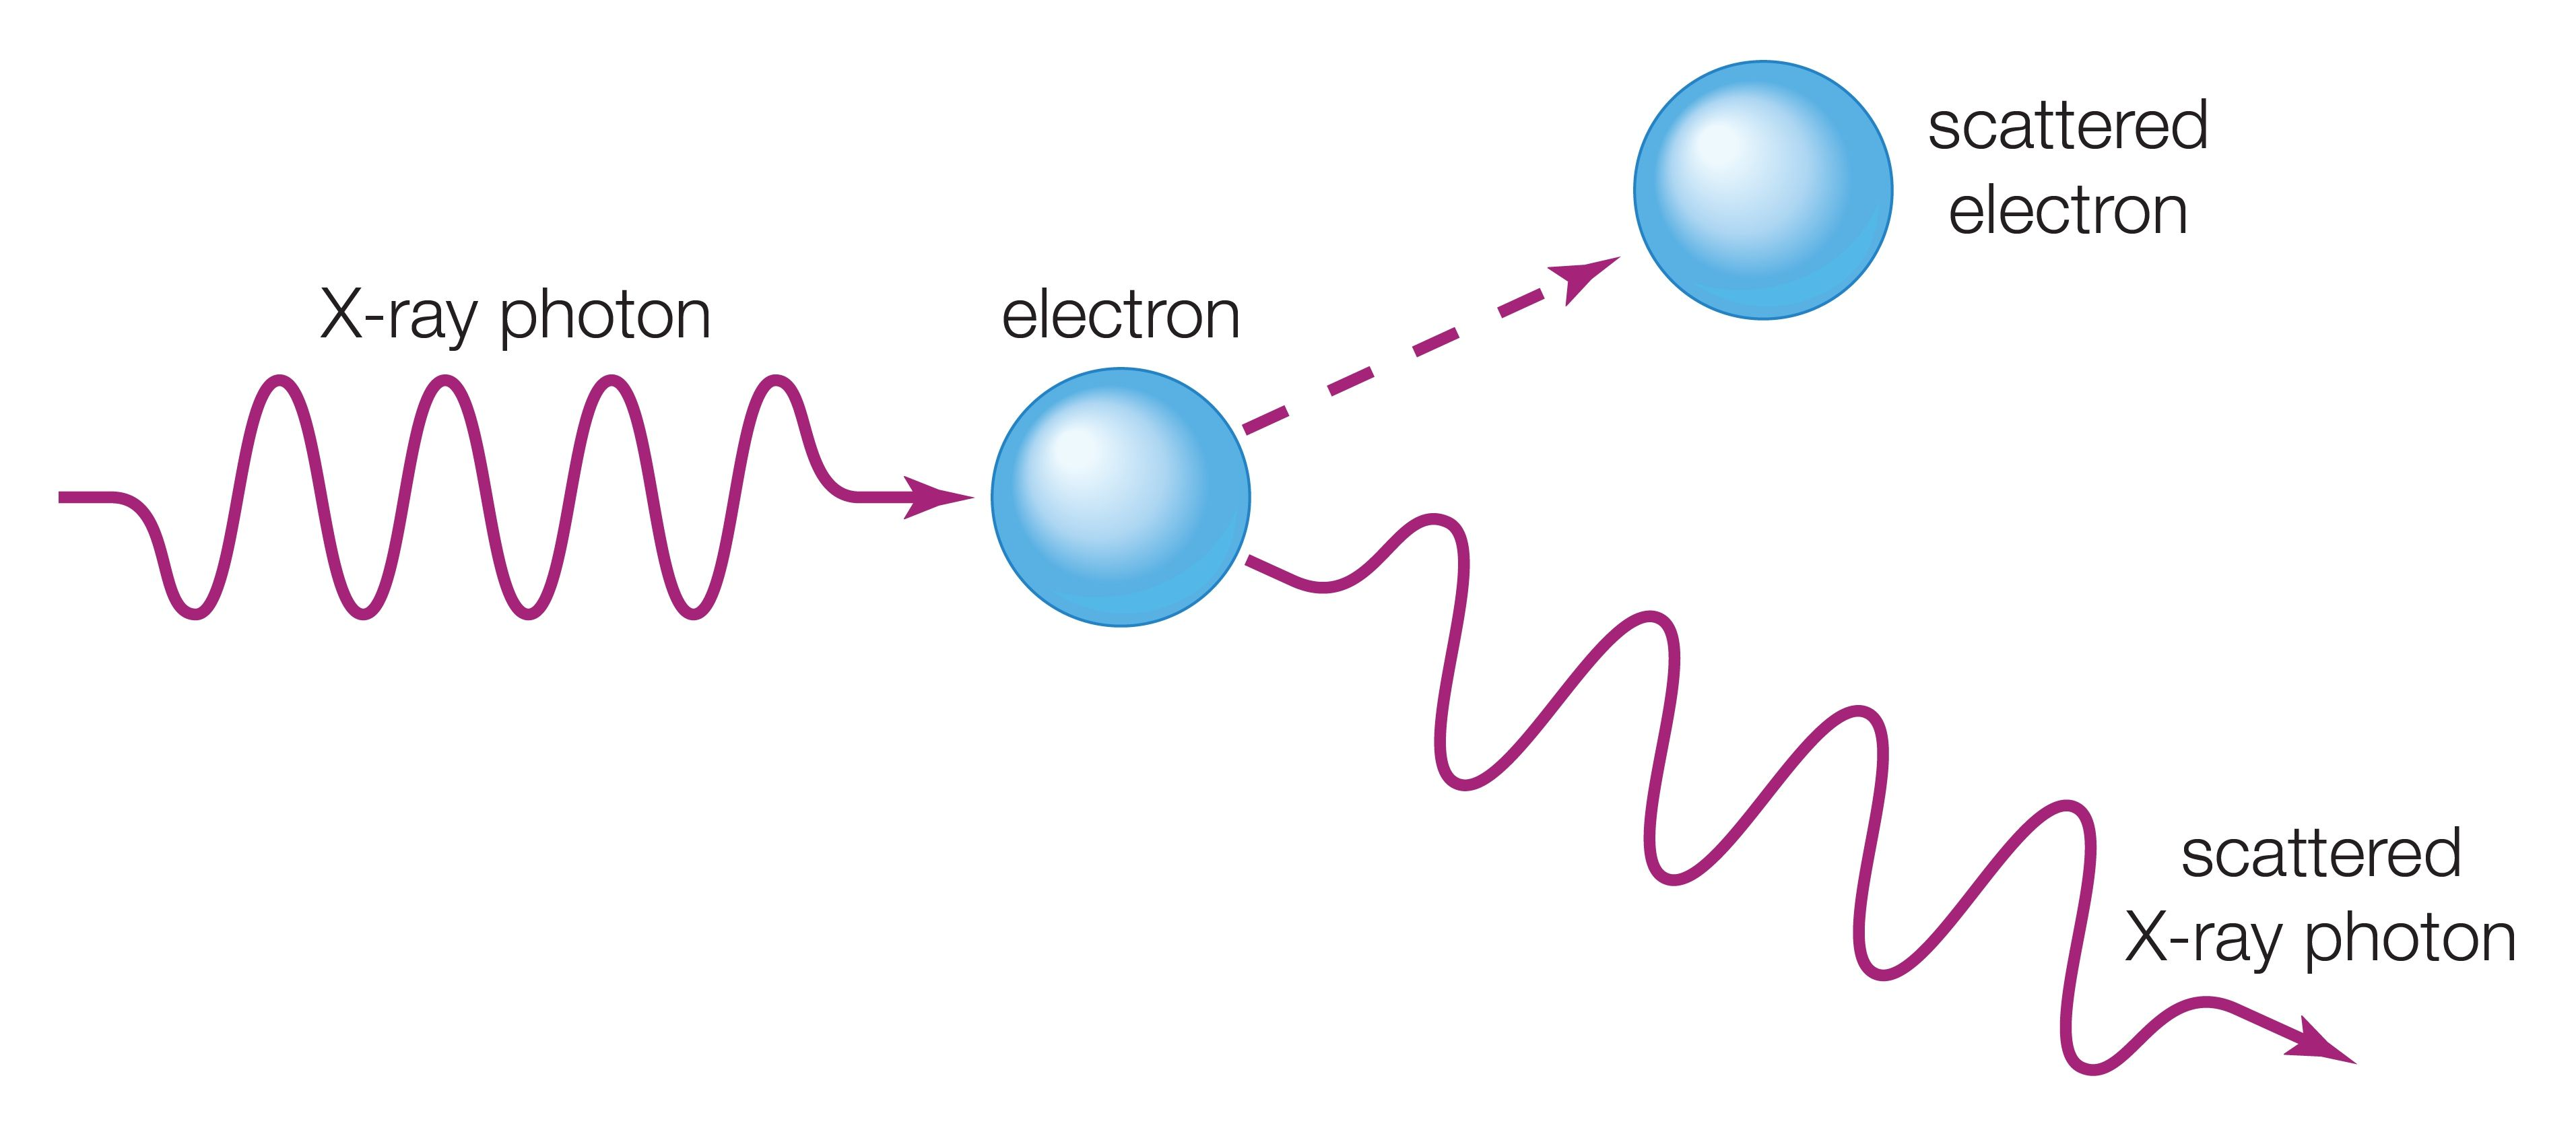
\includegraphics[scale=0.08]{comp.jpg}\\
Protože je mnohem jednoduší detekovat foton než elektron, parametry elektronu vyvodíme z vlastnotí rozptýleného fotonu.
$$p_{1} = p_{2} + p_{e}$$
Na vztah pro comptův rozptyl můžeme přijít ze zákona zachování energie, kde $p_{1}$ je hybnost fotonu před srážkou, $p_{2}$ je hybnost fotonu po srážce a $p_{e}$ je hybnost elektronu.\\
Nesmíme zapomenout, že hybnosti jsou vektory. Dále v textu už notaci vektorů nepoužívám.
$$(\vec{p}_{1} - \vec{p}_{2})^{2} = \vec{p}_{1}^{2} \vec{p}_{2}^{2} -2\vec{p}_{1}\vec{p}_{2}$$
$$(\vec{p}_{1} - \vec{p}_{2})^{2} = \vec{p}_{1}^{2} \vec{p}_{2}^{2} -2p_{1}p_{2}cos(\theta)$$
Potom bude úhel $\theta$ úhel rozptylu fotonem před srážkou a po srážce.\\
Pokud elektron bude před srážkou v klidu, bude mít energii $E_{0} = mc^{2}$, po srážce bude
mít energii $\sqrt{E_{0} + p^{2}_{e}c^{2}}$.
$$p_{1}c + E_{0} = p_{2}c + \sqrt{E_{0}^{2} + p_{e}^{2}c^{2}}$$
$$\vdots$$
\begin{equation}\label{eq:1}
  \lambda_{1} - \lambda_{2} = \frac{h}{m_{0}c} (1-cos\theta)
\end{equation}
$\lambda_{1}$ je vlnová délka nalétavajícího fotonu a $\lambda_{2}$ fotonu po srážce.\\
Vydělením předchozí rovnice $h$ dostaneme vztah\\
$$\frac{1}{h} (\lambda_{1} - \lambda_{2}) = \frac{1}{m_{0}c} (1-cos\theta)$$
$$\frac{1}{p_{1}} - \frac{1}{p_{2}} = \frac{1}{m_{0}c} (1-cos\theta)$$
Vydělím celou rovnici $c$\\
\begin{equation}\label{eq:2}
  \frac{1}{E_{1}} - \frac{1}{E_{2}} = \frac{1}{m_{0}c^{2}} (1-cos\theta)
\end{equation}
\section{Postup měření}
Na stole byl detektor a zdroj záření umístěny proti sobě pod úhlem $180^{\degree}$.\\
Detektor byl zapnut a data byla odesílána do počítače.\\
Snímal jsem 10 sekund a uložil data.\\
Posunul jsem dekektor o $10^{\degree}$ a opakoval jsem proces.\\
Detektor jsem celkově posouval pro úhly od $0^{\degree} - 70^{\degree}$.
\newpage
\section{Data}
\begin{figure}[h]
  \hspace*{-1em}
  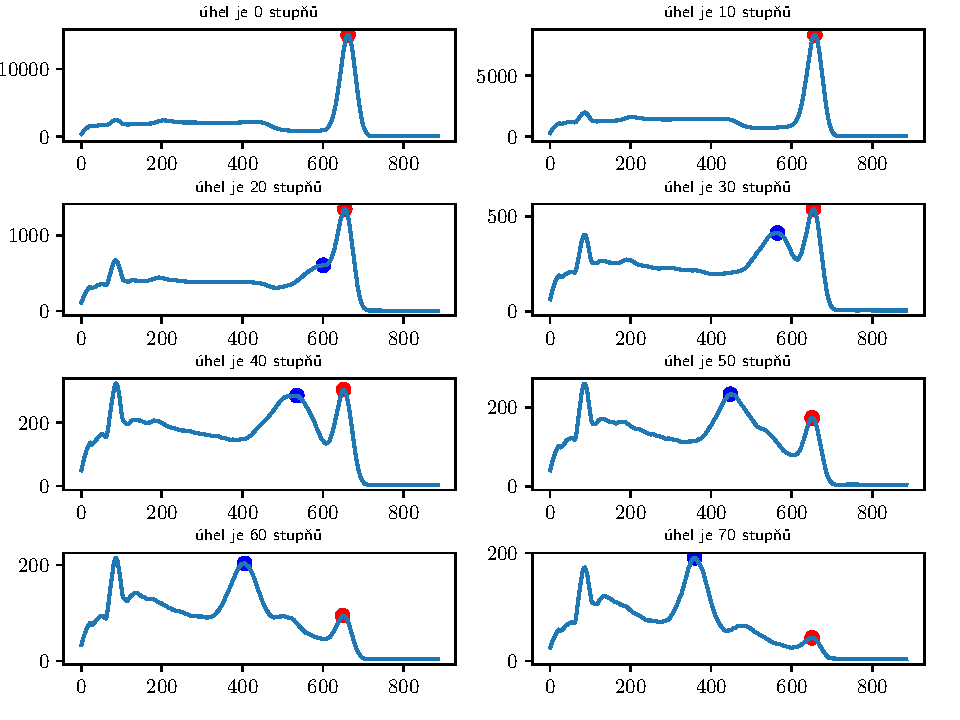
\includegraphics[scale=0.8]{figs/fig1.pdf}
  \caption{Graf závislosti napětí odezvy vzorku na napětím budícím magnetické pole}
\end{figure}
\\
Jednotlivé peaky v grafu značí energii $E_{2}(\lambda_{2})$ (ten modrý) a $E_{1}(\lambda_{1})$ (ten červený).\\
\\
\footnotesize{Tabulka 1:}\\

\csvreader[
tabular = |c|c|c|c|,
table head =
\hline
{úhel}&{$E_{2}[KeV]$}&{$E_{1}[KeV]$}&{$1 - cos(\theta)$}\\
\hline
\hline,
late after line = \\\hline
]{figs/data1.csv}{}{
  \csvcoli & \csvcolii & \csvcoliii & \csvcoliv}
\\
\vspace{1em}
\\
$E_{1}$ je konstantní. Když jsem hodnoty zprůměroval, vyšlo mi\\
$\overline{E_{1}} = 653.659 \pm 4.118$, což však není přesná hodnota.
\newpage
\\
Rovnici \ref{eq:2} můžeme upravit na tvar\\
$$- \frac{1}{E_{2}} = \frac{1}{m_{0}c^{2}} (1-cos\theta) - \frac{1}{E_{1}}$$
$$\frac{1}{E_{2}} = -\frac{1}{m_{0}c^{2}} (1-cos\theta) + \frac{1}{E_{1}}$$
Což je vlastně lineární rovnice o tvaru $u(x) = -ax + b$
\begin{figure}[h]
  \hspace*{-1em}
  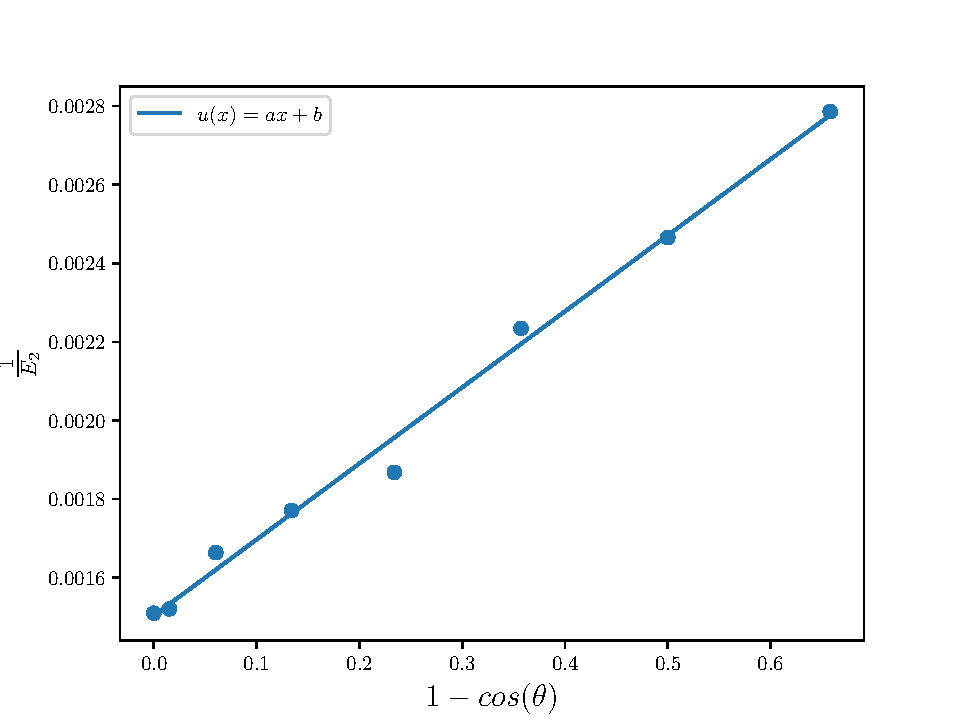
\includegraphics[scale=0.8]{figs/fig2.pdf}
  \caption{Graf závislosti napětí odezvy vzorku na napětím budícím magnetické pole}
\end{figure}
\\
Kde $a = 0.00193438$ a $b = 0.00150388$\\
$$a = \frac{1}{m_{0}c^{2}}$$
$$m_{0} = \frac{1}{ac^{2}} = 516.961 \frac{KeV}{c^{2}} = 9.215 \cdot 10^{-31} Kg$$
$$b = \frac{1}{E_{1}}$$
$$E_{1} = \frac{1}{b} = 664.943 KeV$$
\newpage
\section{Diskuse}
Jak je vidět z grafů a tabulek, energie gamma ($E_{2}$) klesá v závislosti na úhlu rozptylu.
Vykreslil jsem graf $\frac{1}{E_{2}}(1-cos\theta)$, ze kterého jsem potom určil původní
energii gamma a klidovou hmotnost elektronu. Naměřené hodnoty s však od tabulkových
hodnot liší. Chyba mohla být vytvořena nepřesným umístěním detektoru pod správný úhel.
\section{Závěr a naměřené hodnoty}
$$m_{0} = 9.215 \cdot 10^{-31} [Kg]$$
$$E_{1} = 664.943 [KeV]$$
\section{Zdroje}
\url{https://phys.libretexts.org/Bookshelves/Modern_Physics/Book%3A_Spiral_Modern_Physics_(D'Alessandris)/4%3A_The_Photon/4.2%3A_Compton_Scattering}\\\\
\url{https://courses.physics.ucsd.edu/2017/Spring/physics4e/compton.pdf}
\end{document}
